\documentclass[journal]{IEEEtran}

\usepackage{amsmath,amssymb,amsfonts}
\usepackage{graphicx}
\usepackage{textcomp}
\usepackage{xcolor}
\usepackage{booktabs}
\usepackage{multirow}
\usepackage{array}
\usepackage{tabularx}
\usepackage{cite}
\usepackage{url}
\usepackage{listings}
\lstset{
    basicstyle=\ttfamily\footnotesize,
    breaklines=true,
    breakatwhitespace=false,
    columns=fullflexible,
    keepspaces=true,
    showstringspaces=false,
    aboveskip=0.7em,
    belowskip=0.7em,
    frame=single,
    rulecolor=\color{black!20},
    xleftmargin=0.3em,
    xrightmargin=0.3em
}
\emergencystretch=1em

\begin{document}

\title{Networking for DevOps:\\From Fundamentals to Secure Services}
\author{Mohammad Fatahi}
\markboth{Networking for DevOps}{From Fundamentals to Secure Services}
\maketitle

\begin{abstract}
This chapter explains the network concepts behind common DevOps tasks and connects them to practical Linux commands. It begins with communication layers, addressing, routing, and network configuration, then examines troubleshooting, firewall management, and performance. HTTP, HTTPS, FTP, DNS, and SSH examples show how services use these foundations. The final sections introduce monitoring and a systematic approach to diagnosing failed or slow connections.
\end{abstract}
\begin{IEEEkeywords}
Linux networking, DevOps, TCP/IP, DNS, HTTP, TLS, SSH, troubleshooting.
\end{IEEEkeywords}

\section{Introduction}
A web page can appear simple from the user's perspective: enter an address and wait for a response. Behind that action, several things must work together. The computer needs a network connection and an address, the name must resolve, packets need a route, a service must listen on the right port, and the application must return an appropriate response. If HTTPS is used, the client also needs to verify the server and establish an encrypted connection.

The question then arises: where should a DevOps engineer begin when one of these steps fails? The answer starts with understanding the responsibility of each part of the network. This chapter therefore introduces the basic concepts first and then follows them through configuration, service deployment, security, monitoring, and troubleshooting. The examples use Linux tools so that each explanation can be connected to an observable result.

The practical examples follow the topics of two networking exercise sets: basic network configuration and diagnostics, followed by common services and more detailed troubleshooting. Commands are examples to run in a suitable laboratory, not measurements already collected from a particular machine. Interface names, addresses, usernames, and service names should be checked against the actual environment. We will also distinguish what a successful test proves from what still needs to be investigated.

\section{Data Communication and Networking}

The first concept we should get familiar with is a network. A network allows multiple devices to exchange data with each other via a communication medium. Communication media include copper cables, optical fiber, and air (for Wi-Fi and radio waves). In network communication, we have a client and a server. A client is typically the one who requests a service. A server is a system that provides a service.

The question then arises: what types of networks do we commonly encounter? Examples include LAN (Local Area Network), such as the home network; WAN (Wide Area Network), such as a company that has two offices in Tehran and Montreal; these two LANs can be connected to each other via WAN, and the Internet, which interconnects many networks. These examples are not an exhaustive classification. Open Systems Interconnection Model (OSI model) is a seven-layer conceptual model that explains the responsibility of each part of a network when two devices communicate over a network. This conceptual model is illustrated in Fig.~\ref{fig:osi_model}. At the highest layer, we have the application layer, which has protocols for addressing the demands raised by applications like Google Chrome. As illustrated in Fig.~\ref{fig:application_layer}, different protocols exist in the seventh layer. Some of these are as follows:

\begin{itemize}
    \item \textbf{HTTP/HTTPS:} These protocols enable communication between web clients and web servers, with HTTPS providing encrypted and secure data exchange using TLS.
    \item \textbf{DNS:} This protocol translates human-readable domain names, such as \texttt{example.com}, into IP addresses required for locating hosts on a network.
    \item \textbf{SMTP:} This protocol is primarily used for sending and transferring email messages from clients to mail servers and between mail servers.
    \item \textbf{IMAP:} This protocol allows users to access, manage, and synchronize email messages stored on a remote mail server across multiple devices.
    \item \textbf{SSH:} This protocol provides secure encrypted remote access to computers and servers for command execution, administration, and remote management.
    \item \textbf{FTP:} This protocol is used to transfer files between a client and a server over a network, supporting operations such as uploading, downloading, and file management.
\end{itemize}


\begin{figure}[t]
    \centering
    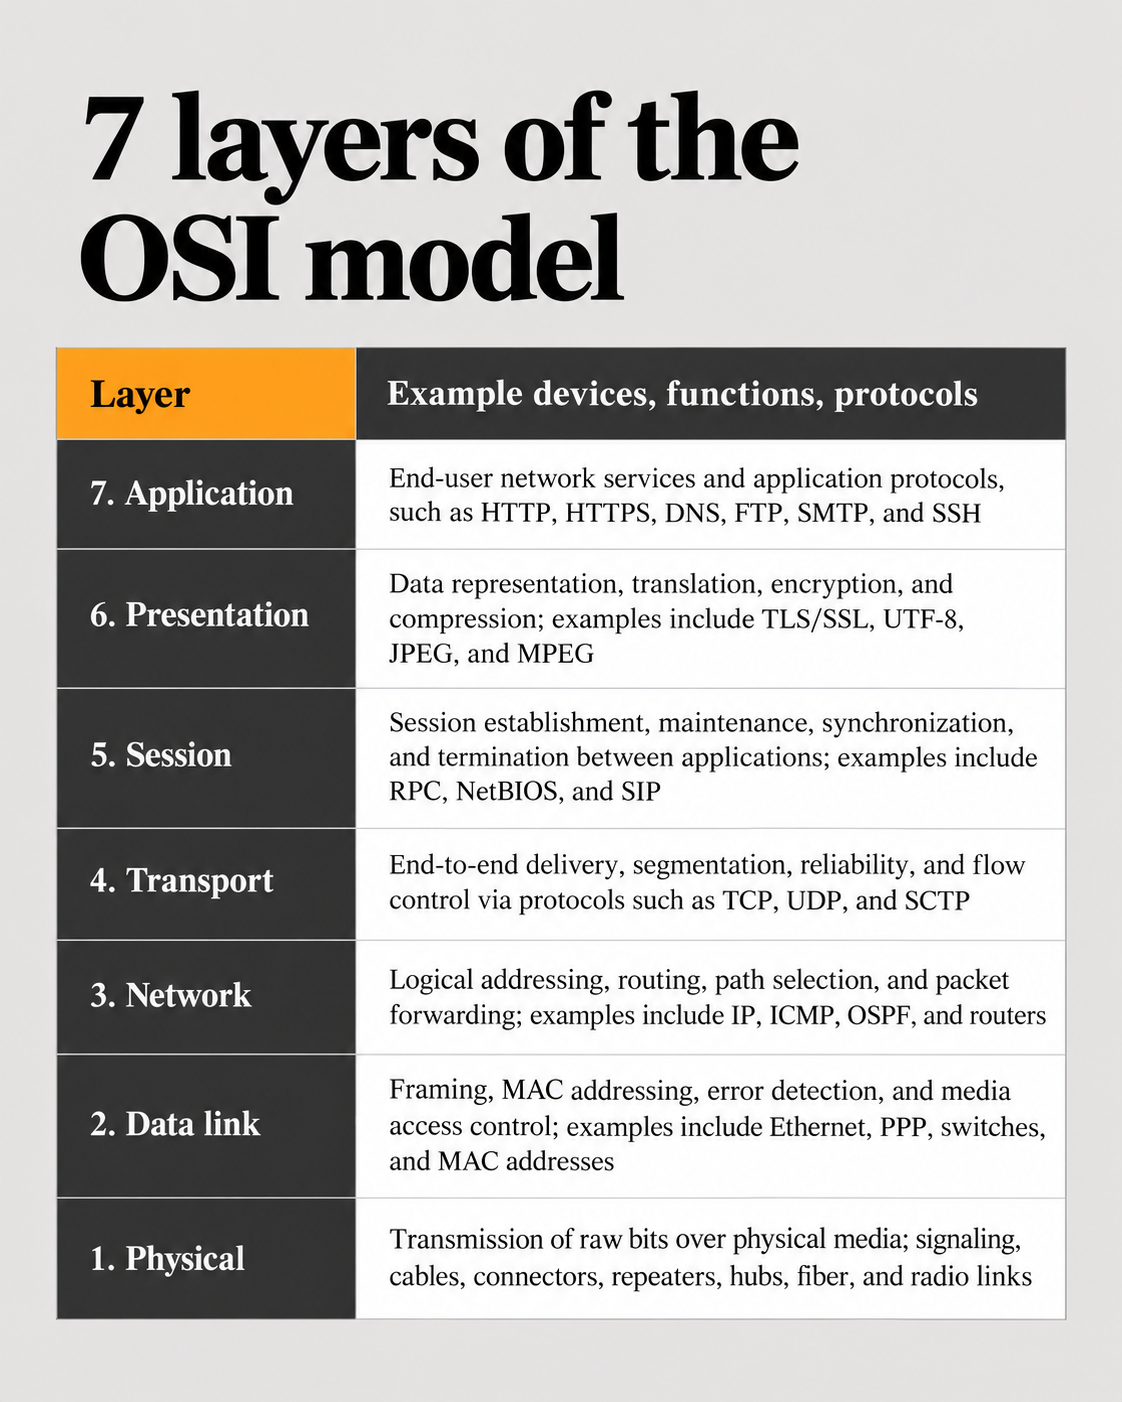
\includegraphics[width=\linewidth]{images/1.png}
    \caption{The seven layers of the OSI model, illustrating the primary functions, protocols, and networking components associated with each layer.}
    \label{fig:osi_model}
\end{figure}

\begin{figure*}[t]
    \centering
    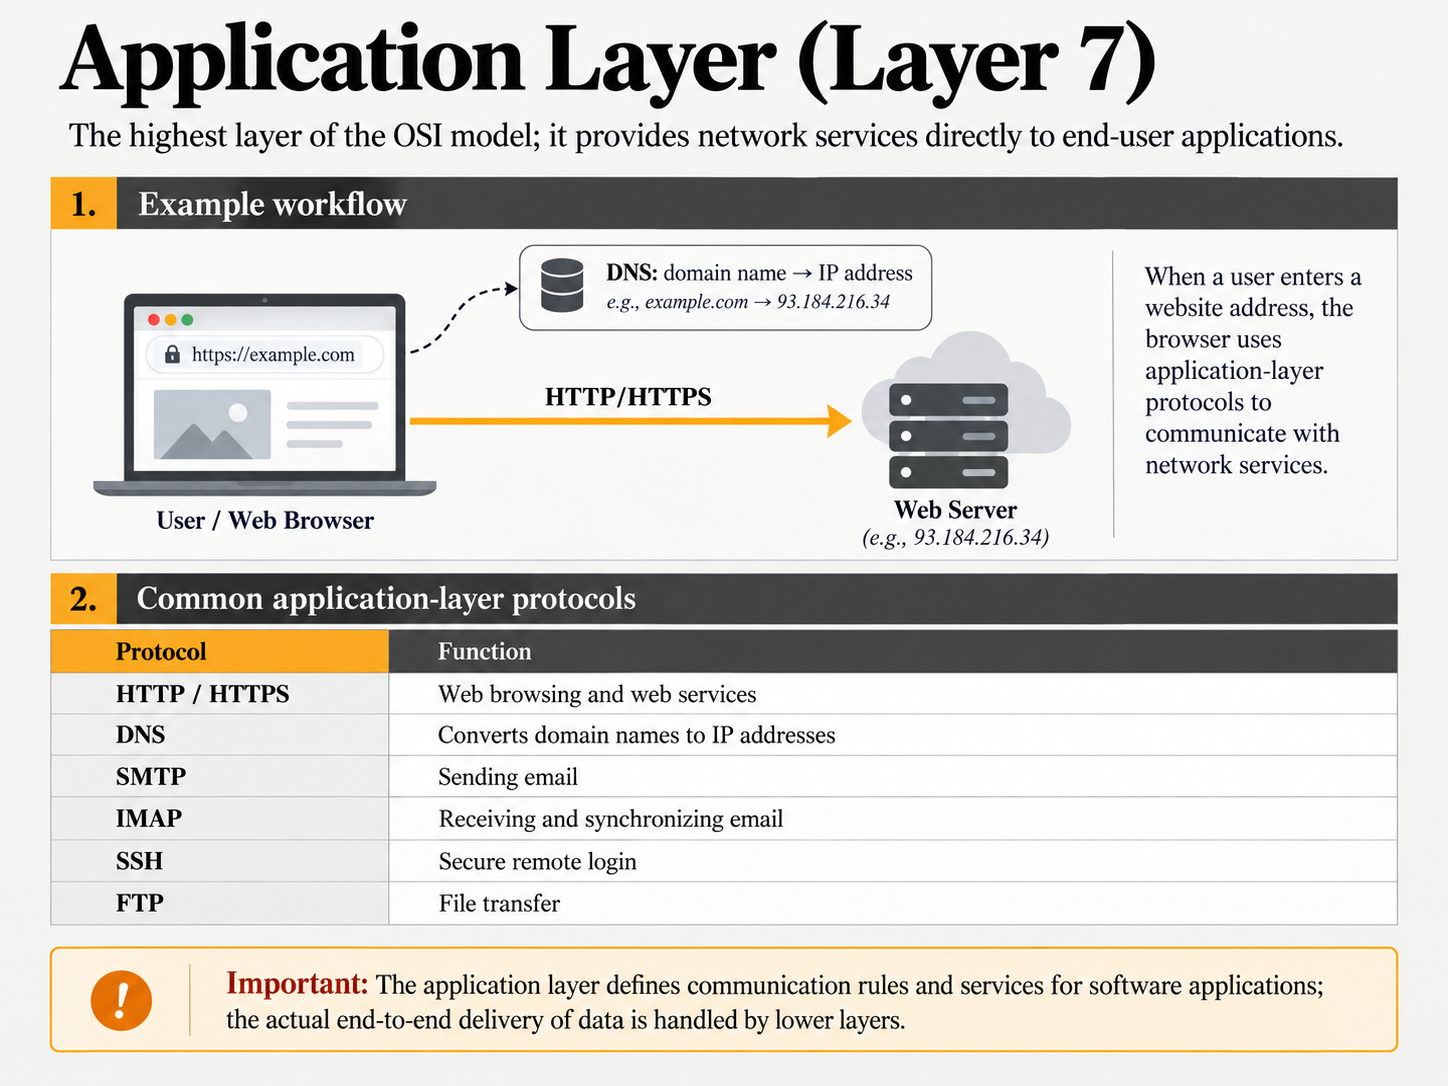
\includegraphics[width=\textwidth]{images/2.png}
    \caption{Overview of the OSI application layer (Layer 7), illustrating a typical web communication workflow and common application-layer protocols and their functions.}
    \label{fig:application_layer}
\end{figure*}

After the Application Layer, where clients express their requests through protocols such as HTTPS, the next step is to define how the request data is formatted, represented, and encoded for communication. This step is handled by the \textbf{Presentation Layer}. Its role is to ensure that data is represented in a format that can be correctly interpreted by the receiving system. For example, the text \textbf{"Hello"} can be encoded into a binary representation using a character-encoding standard such as UTF-8. Common data representation and encoding formats include \textbf{UTF-8, JPEG, PNG, JSON, and XML}. In the next layer (Layer 5: Session), a communication session is established and managed between two applications, allowing them to maintain an organized and continuous exchange of data. In modern real-world networks, the boundaries between OSI Layers 5, 6, and 7 (Session, Presentation, and Application) are not always clearly defined. Therefore, in the TCP/IP model, the functions of these three OSI layers are generally combined into a single layer known as the \textbf{Application Layer}. The next layer is the \textbf{Transport Layer}, one of the most important layers in network communication. This layer is responsible for communication between processes and applications on two computers. There are three important protocols in the transport layer, which are as follows:


\begin{itemize}
    \item \textbf{TCP (Transmission Control Protocol):} TCP is a connection-oriented and reliable transport protocol that provides an ordered byte stream, detects missing data, and retransmits when necessary. A connection can still fail; reliability does not guarantee that an unavailable destination will receive the data.

    \item \textbf{UDP (User Datagram Protocol):} UDP is a connectionless transport protocol that sends data without establishing a connection or guaranteeing delivery, ordering, or retransmission. Its lower transport overhead can make it suitable for delay-sensitive applications such as real-time streaming, VoIP, and online gaming.

    \item \textbf{SCTP (Stream Control Transmission Protocol):} SCTP is a reliable, message-oriented transport protocol that supports features such as multi-streaming and multi-homing. It allows multiple independent data streams within one association and can use multiple network paths to improve communication resilience.
\end{itemize}


The next layer is the \textbf{Network Layer}, which is responsible for transmitting messages from one network to another network. The main ideas in this layer are IP Address and Internet Control Message Protocol (ICMP) protocol. While the Transport Layer is responsible for providing appropriate data transmission services based on application requirements, the Network Layer is responsible for logical addressing and routing packets from the source to the destination across interconnected networks. The main concepts of this layer are as follows:


\begin{itemize}
    \item \textbf{IP Address:} An IP address is a logical address assigned to a device on a network and is used to identify the source and destination of IP communication. For example, \texttt{192.168.1.10} can represent a device within a local network.

    \item \textbf{IPv4 and IPv6:} IPv4 and IPv6 are the two main versions of the Internet Protocol. IPv4 uses 32-bit addresses such as \texttt{192.168.1.10}, whereas IPv6 uses 128-bit addresses such as \texttt{2001:db8::1}, providing a significantly larger address space.

    \item \textbf{Private IP Address:} A private IP address is used to identify devices within private networks such as home, office, or enterprise networks and is not directly routable on the public Internet. Common private IPv4 ranges include \texttt{10.0.0.0/8}, \texttt{172.16.0.0/12}, and \texttt{192.168.0.0/16}.

    \item \textbf{Public IP Address:} A public IP address is used to identify Internet-connected endpoints. Public IP addresses must be globally unique while assigned and are typically allocated through Internet service providers or other address-allocation mechanisms.

    \item \textbf{Loopback and Localhost:} A loopback address allows a device to communicate with itself and is commonly represented by \texttt{127.0.0.1} in IPv4. The hostname \texttt{localhost} typically resolves to a loopback address and is commonly used for testing locally running network services.

    \item \textbf{Subnet Mask:} A subnet mask determines which bits of an IPv4 address represent the network portion and which represent the host portion. For example, \texttt{255.255.255.0}, equivalent to \texttt{/24}, indicates that the first 24 bits identify the network.

    \item \textbf{NAT (Network Address Translation):} NAT is a mechanism commonly implemented by routers to translate private IP addresses used within a local network into public IP addresses and vice versa. It allows multiple devices on a private network to access external networks using a shared public IPv4 address.

    \item \textbf{Network Address:} A network address identifies an entire network or subnet rather than an individual host. For example, in the network \texttt{192.168.1.0/24}, \texttt{192.168.1.0} is the network address.

    \item \textbf{Broadcast Address:} A broadcast address is used to send data to all hosts within an IPv4 subnet. For example, the broadcast address of the network \texttt{192.168.1.0/24} is \texttt{192.168.1.255}.

    \item \textbf{Default Gateway:} A default gateway is the router or next-hop address to which a device sends packets destined for networks outside its local subnet. It therefore provides a path from the local network to other networks, such as the Internet.

    \item \textbf{ICMP and Ping:} ICMP (Internet Control Message Protocol) is a Network Layer protocol used for error reporting and network diagnostic messages. The \texttt{ping} utility typically sends ICMP Echo Request messages and receives Echo Reply messages to test reachability and measure round-trip time.

    \item \textbf{Router:} A router is a Network Layer (Layer 3) device that connects different networks and forwards packets between them. It examines destination IP addresses and uses its routing table to determine the appropriate next hop or outgoing path.
\end{itemize}


Now that we are familiar with the layers responsible for expressing a client's request and identifying the source and destination addresses, it is time to examine how data is physically transmitted across a local network and the Internet. The Data Link Layer is responsible for data transmission within a local network. The key concepts of this layer are as follows:

\begin{itemize}
    \item \textbf{MAC Address (Media Access Control Address):} A MAC address is a Layer 2 identifier associated with a network interface and is used for local frame delivery within a network segment. A traditional Ethernet MAC address is 48 bits long and is commonly represented in hexadecimal form, such as \texttt{00:1A:2B:3C:4D:5E}.

    \item \textbf{Ethernet:} Ethernet is a widely used family of technologies for wired local area networks (LANs) and operates primarily at the Data Link and Physical layers. At Layer 2, it defines the Ethernet frame format and uses source and destination MAC addresses to deliver frames across the local network.

    \item \textbf{Switch:} A switch is primarily a Layer 2 network device that connects devices within a LAN and forwards Ethernet frames toward the appropriate port. It learns source MAC addresses to build a MAC address table and uses the destination MAC address of each frame to make forwarding decisions.

    \item \textbf{ARP (Address Resolution Protocol):} ARP is used in IPv4 networks to discover the MAC address associated with an IPv4 address on the local network.

    \item \textbf{ARP Cache:} An ARP cache is a table maintained by a host that temporarily stores mappings between IPv4 addresses and their corresponding MAC addresses. This prevents the host from having to perform a new ARP exchange every time it communicates with the same local destination or next hop.
\end{itemize}


The last layer is the \textbf{Physical Layer}. It deals with signals and the communication medium: copper cables, optical links, and radio transmission. A disconnected cable or weak wireless link can prevent higher layers from working even when their configuration is correct. On a wired interface, \texttt{ip link} and \texttt{ethtool enp0s3} can help inspect carrier and negotiated link settings.

ARP resolves the IPv4 address of a local destination or next hop. If the destination is outside the subnet, the host normally needs the gateway's MAC address rather than the remote server's MAC address. The remote IP address stays in the IP packet while the Layer 2 addresses change as the packet crosses routed links.

\section{Web Server and Network Configuration}
One of the most important applications of computer networks is providing access to web-based services through web servers, which is illustrated in Fig.~\ref{fig:web_server}. A web server receives and processes HTTP or HTTPS requests from clients and returns the appropriate resources or responses. By convention, HTTP services typically listen on TCP port 80, while HTTPS services use TCP port 443. Other network services use their own well-known ports; for example, SSH commonly uses TCP port 22, while DNS typically uses port 53 over UDP or TCP, depending on the operation.

NGINX is a widely used, cross-platform web server that can receive and process HTTP/HTTPS requests and deliver web content to clients. However, deploying a web server involves more than simply installing web-server software. Proper network configuration is also required to ensure that the server is correctly addressed, reachable by clients, and accessible through the required network ports.

\begin{figure*}[t]
    \centering
    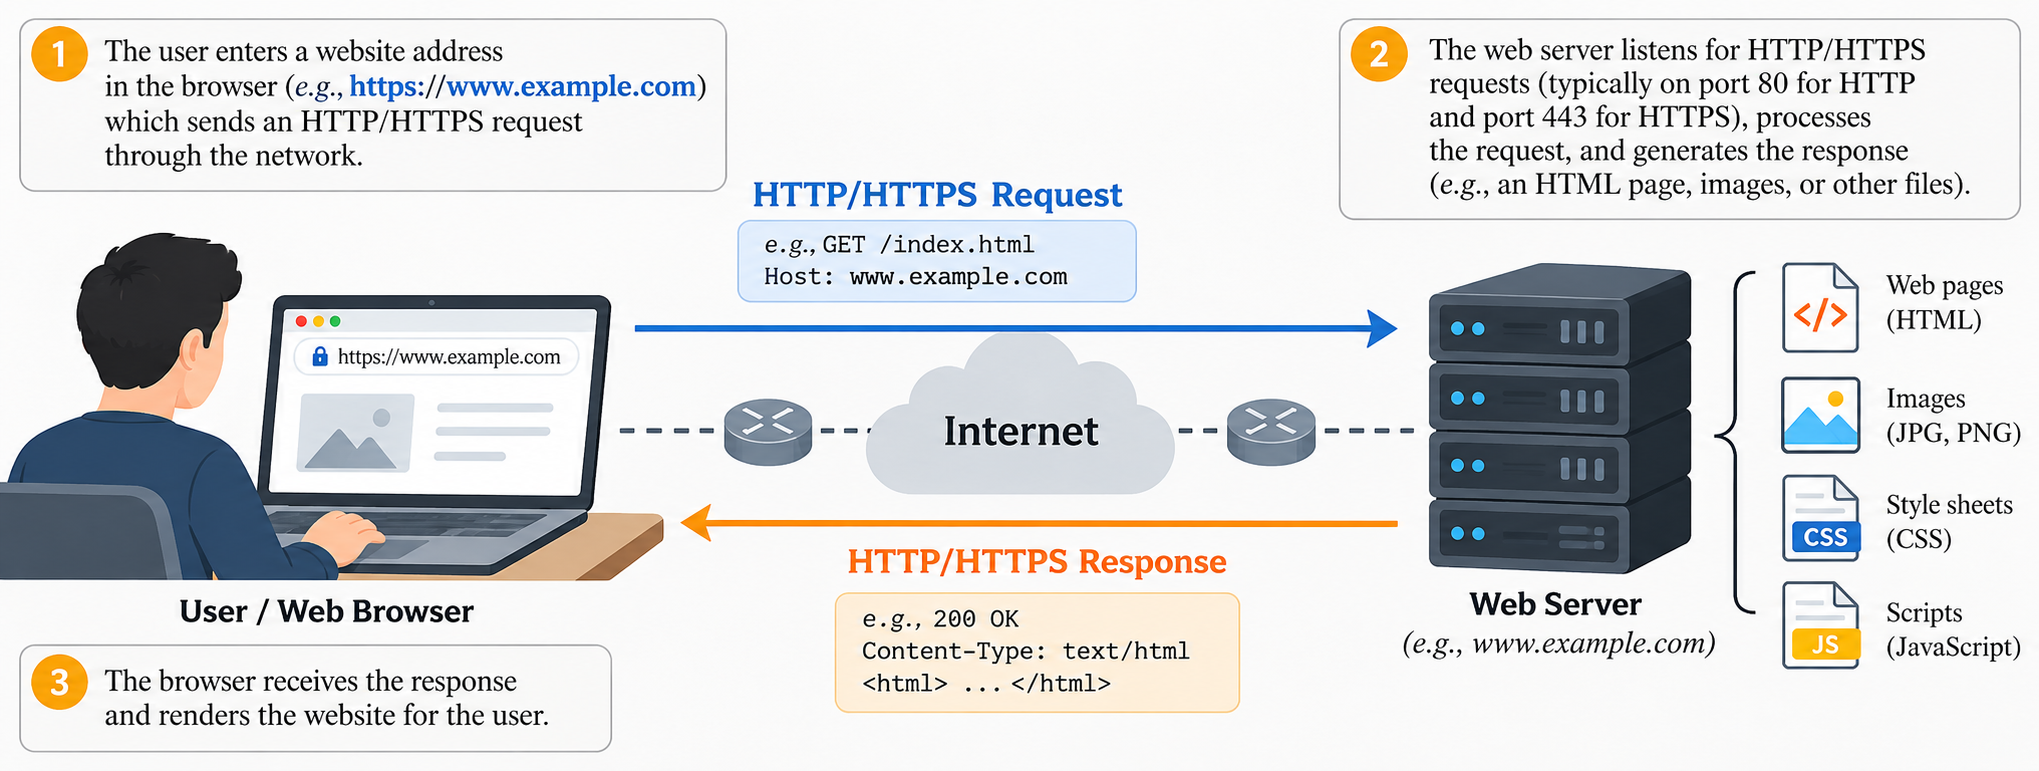
\includegraphics[width=\textwidth]{images/3.png}
    \caption{Conceptual illustration of web-based communication, where a user sends an HTTP/HTTPS request through the Internet to a web server, which processes the request and returns the requested web content as an HTTP/HTTPS response.}
    \label{fig:web_server}
\end{figure*}

\subsection{Basic Network Configuration}
The first step in configuring a web server is to verify its basic network configuration. The basic network configuration includes the following steps:
\begin{enumerate}
    \item Checking network interfaces.
    \item Checking the assigned IP address.
    \item Checking the default gateway.
    \item Checking DNS servers.
\end{enumerate}

The first step is to verify the network interfaces and assigned IP addresses. This can be done by executing the \texttt{ip addr} or \texttt{ip link} commands in the command line. Network interfaces represent all possible networks to which a specific device can connect based on its hardware and software, encompassing both virtual tunnels (such as Tailscale) and physical connections (such as Wi-Fi or Ethernet). Both physical and virtual interfaces can report administrative and operational states. A virtual interface may show \texttt{UNKNOWN} because its link does not behave like a physical carrier; this does not alone establish that the interface is unusable. The output of the \texttt{ip addr} command yields comprehensive details regarding all configured network interfaces on the device, including their assigned IP addresses and hardware (MAC) addresses. After identifying these available interfaces and their respective IP addresses, the next step is to examine the default gateway using the \texttt{ip route} command. So far, we have identified available interfaces and their characteristics for a device and how the device can send its request to  the destination whether it is in the local network or not. Resolving a destination name usually involves DNS, although a local hosts-file entry may provide the answer without a DNS query. Some Linux systems use a local DNS stub resolver that forwards queries to upstream DNS servers; other configurations query upstream servers directly. When an application requires DNS resolution to determine a destination IP address, it may send its query to the local DNS stub resolver, which forwards the request to the appropriate upstream DNS server. To identify the local stub resolver, one can examine the \texttt{/etc/resolv.conf} file. On a system using systemd-resolved, \texttt{resolvectl status} displays per-link resolver information, including upstream DNS servers.


The question then arises: how is an IP address assigned to a device within a network? Two common approaches are dynamic assignment through DHCP and static configuration. A DHCP server offers configuration to a client; the server may run on a router or on another system. Receiving an address also depends on the client, network connectivity, and available leases.

\subsection{Static Configuration with Netplan}
On systems that use Netplan, YAML files describe the intended network configuration. A renderer, commonly systemd-networkd or NetworkManager, manages the interface using the generated configuration. First inspect the existing files in \texttt{/etc/netplan} and identify which component owns the interface. Files can be merged, so adding a second file without checking existing definitions may leave conflicting settings.

For a laboratory interface named \texttt{enp0s3}, a static configuration can be:
\begin{lstlisting}
network:
  version: 2
  renderer: networkd
  ethernets:
    enp0s3:
      dhcp4: false
      addresses:
        - 192.168.1.100/24
      routes:
        - to: default
          via: 192.168.1.1
      nameservers:
        addresses: [8.8.8.8, 1.1.1.1]
\end{lstlisting}
Use spaces for indentation, and replace the interface and addresses with values suitable for the real network. The static address should not conflict with another host or an unmanaged DHCP allocation. Netplan's examples show the same separation between addresses, routes, and DNS configuration~\cite{netplan}.

\begin{figure*}[t]
    \centering
    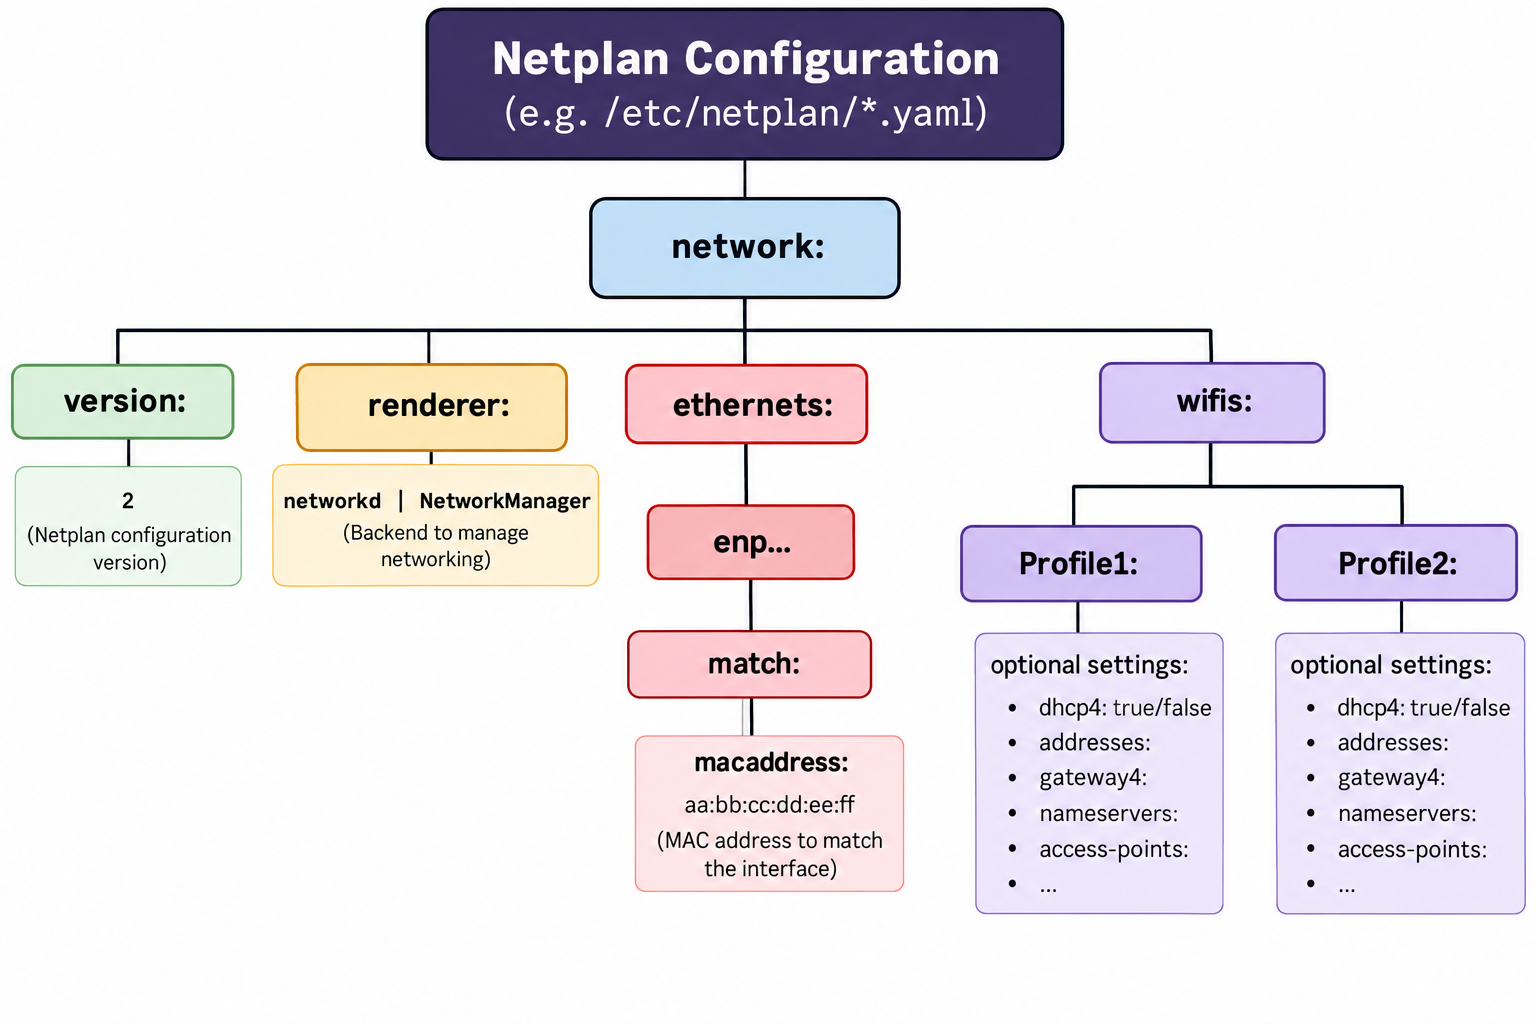
\includegraphics[width=0.9\textwidth]{images/4.png}
    \caption{The structure of a Netplan configuration. The diagram includes the older gateway4 field; the example in this chapter expresses the default gateway through routes.}
    \label{fig:netplan}
\end{figure*}

Save the reviewed configuration in an appropriate file under \texttt{/etc/netplan}, restrict its permissions, and inspect it before applying:
\begin{lstlisting}
sudo chmod 600 /etc/netplan/01-lab.yaml
sudo netplan generate
sudo netplan get
sudo netplan try
\end{lstlisting}
\texttt{generate} creates the renderer configuration and detects many syntax problems. \texttt{get} displays the merged settings; it does not apply them. \texttt{try} applies settings temporarily and asks for confirmation, with rollback if they are not confirmed. Verify the result before confirming, especially on a remote server. \texttt{sudo netplan apply} applies configuration directly. Restarting NetworkManager is not a universal additional step because the selected renderer may be systemd-networkd.

\subsection{Verifying the Configuration}
After configuration, inspect the interface, routes, resolver, and reachability:
\begin{lstlisting}
ip -br addr
ip route
resolvectl status
ping -c 5 8.8.8.8
ping -c 5 google.com
nslookup github.com
ss -ltnp
ss -tn state established
\end{lstlisting}
If the numeric destination is reachable but name resolution fails, investigate DNS. If ping fails, do not immediately conclude that the web service is unavailable: ICMP may be blocked even when TCP is allowed. Socket inspection shows local endpoints and states, while the process details may require \texttt{sudo}.

\section{Routing and Network Topology}
The question then arises: how does a packet leave the local network? A host consults its routing table and chooses the matching route with the most specific destination prefix. The default route is used when no more specific route matches.
\begin{lstlisting}
ip route
ip route get 8.8.8.8
ip neigh
traceroute 8.8.8.8
mtr -r -c 10 8.8.8.8
\end{lstlisting}
\texttt{ip route} shows the local routing table. \texttt{ip route get} shows the selected route and source address for a destination. \texttt{ip neigh} shows neighbor information. Traceroute and mtr probe the path beyond the local host; they are not substitutes for the routing table.

An asterisk in traceroute means that the probe did not receive the expected reply within the timeout. Routers may filter or limit diagnostic responses while still forwarding application traffic. Similarly, loss at an intermediate mtr hop is not proof of forwarding loss when subsequent hops answer normally. Compare the final destination and repeated observations before identifying a fault.

\subsection{A Small Star Topology}
In a star topology, devices connect to a central switch. One example subnet is \texttt{192.168.1.0/24}: the router uses \texttt{192.168.1.1}, three servers use \texttt{192.168.1.10} through \texttt{192.168.1.12}, and ten computers use \texttt{192.168.1.100} through \texttt{192.168.1.109}. The range ending at \texttt{.110} contains eleven addresses, so that last address can be kept as a spare. The switch provides local connectivity, while the router provides a path to other networks. A managed switch can have a management address; switching frames does not itself require a host IP address on every switch port.

\section{Network Troubleshooting}


This subsection outlines approaches for network troubleshooting. When a web server fails to respond to a client's request, we need a systematic way to identify and resolve the underlying issue.

\begin{enumerate}

    \item \textbf{Verify Listening Ports:}
    The first step is to check if the web server is actively listening on HTTP (80) and HTTPS (443). We can verify this using the following command:
    \begin{lstlisting}
sudo ss -ltnp '( sport = :80 or sport = :443 )'
    \end{lstlisting}
    A listening socket confirms that a process accepts connections at that local endpoint. Check its bind address and test the application response; listening alone does not prove application health or external accessibility.

    \item \textbf{Analyze Network Traffic:}
    To evaluate the connection quality and server-client interaction, we use \texttt{tcpdump} to capture traffic on port 80 across the network interfaces. This shows HTTP-port traffic. Ordinary DNS queries use port 53 and need a separate capture filter.

    A timed capture can be written as:
    \begin{lstlisting}
sudo timeout 30 tcpdump -i any -nn \
  -w http.pcap 'tcp port 80'
sudo timeout 30 tcpdump -i any -nn \
  -w dns.pcap 'port 53'
    \end{lstlisting}
    Generate traffic while the capture runs. Thirty seconds is a duration; \texttt{tcpdump -c 30} would stop after thirty packets instead. DNS over HTTPS is encrypted traffic on a different port and is not exposed by the ordinary DNS filter.

    \item \textbf{Deep Packet Inspection:}
    For a deeper analysis, save the \texttt{tcpdump} output to a \texttt{.pcap} file and open it in Wireshark.
    \begin{itemize}
        \item Navigate to \textbf{Statistics $>$ Conversations} to review the TCP connections.
        \item Apply the \texttt{tcp.analysis.retransmission} display filter to inspect suspected retransmissions. Capture gaps or reordering can affect this classification. Use \texttt{tcp.analysis.ack\_rtt} for observed acknowledgement timing, and the \texttt{dns} filter to inspect queries and replies~\cite{wireshark}.
    \end{itemize}

    \item \textbf{Test Client Accessibility:}
    Finally, to determine if a specific port is actually accessible from the client's perspective, use \texttt{telnet} or \texttt{nc} from the client:
    \begin{lstlisting}
telnet 192.168.1.100 80
nc -vz -w 5 192.168.1.100 22
nc -vz -w 5 192.168.1.100 3306
    \end{lstlisting}
    A successful TCP connection establishes port reachability from that client. It does not authenticate the user or prove that the protocol exchange succeeds.

\end{enumerate}

\subsection{Following the OSI Layers}
The OSI model provides a useful checklist even though real protocols do not always fit its boundaries perfectly:
\begin{enumerate}
    \item \textbf{Physical:} Inspect cable, wireless association, carrier, and link settings.
    \item \textbf{Data Link:} Check the interface MAC address, neighbor table, VLAN, and switch connection.
    \item \textbf{Network:} Check the IP address, subnet, gateway, and selected route; test reachability where ICMP is permitted.
    \item \textbf{Transport:} Check TCP or UDP endpoints, firewall rules, and whether the client can reach the intended port.
    \item \textbf{Session:} Inspect whether an established protocol exchange remains usable or is repeatedly interrupted.
    \item \textbf{Presentation:} Check TLS negotiation, certificate verification, and data encoding where relevant.
    \item \textbf{Application:} Inspect DNS answers, HTTP status codes, service logs, and the application's actual behavior.
\end{enumerate}
Session and presentation functions are often part of the application stack in TCP/IP. The checklist organizes questions; it does not imply that Linux has a separate diagnostic command for every OSI layer.

 \section{Network Security}

Evaluating a system's network security typically involves two primary components:
\begin{enumerate}
    \item \textbf{Firewall Management}
    \item \textbf{Network Monitoring}
\end{enumerate}

A firewall is designed to control access, granting or denying connection permissions to clients and systems based on predefined rules. It can be easily enabled, disabled, and customized to align with an administrator's specific security policies. In Linux environments, the Uncomplicated Firewall (UFW) is commonly used for this purpose.

\subsection{Essential UFW Configuration Commands}

\begin{itemize}

    \item \textbf{Enable, Disable, and Status:}
    To turn the firewall on or off, use \texttt{sudo ufw enable} or \texttt{sudo ufw disable}. To check its current state (active/inactive), run:
    \begin{lstlisting}
sudo ufw status
    \end{lstlisting}

    \item \textbf{Resetting Policies:}
    In an isolated lab, the following command clears existing rules. It is destructive to the current firewall policy and is not a required first step on a configured server:
    \begin{lstlisting}
sudo ufw --force reset
    \end{lstlisting}

    \item \textbf{Setting Default Policies:}
    Define baseline traffic rules according to the access policy. For instance, to block all incoming traffic (creating exceptions later) while allowing all outgoing traffic, use:
    \begin{lstlisting}
sudo ufw default deny incoming
sudo ufw default allow outgoing
    \end{lstlisting}

    \item \textbf{Configuring Exceptions (Ports and Protocols):}
    To allow or deny specific traffic, specify the port number and protocol. For example, to allow HTTP traffic over TCP:
    \begin{lstlisting}
sudo ufw allow 80/tcp
    \end{lstlisting}

    \item \textbf{Restricting Access by Network (Private vs. Public):}
    It is often necessary to grant access exclusively from a private local network rather than the outside internet. To achieve this (e.g., allowing SSH access on port 22 only from a specific local subnet), use a command formatted like this:
    \begin{lstlisting}
sudo ufw allow from 192.168.1.0/24 to any port 22 proto tcp
    \end{lstlisting}
    \textit{Note: Replace \texttt{192.168.1.0/24} with your actual local network subnet.}

\end{itemize}


\subsection{Network Monitoring and Anomaly Detection}

Network monitoring involves actively observing network traffic to understand the current state and behavior of the system. The primary objective of this process is anomaly detection. In a network security context, an anomaly typically falls into one of two categories:

\begin{enumerate}
    \item \textbf{High-Frequency Connections:} An unusually high number of connection attempts or established sessions originating from a single IP address. This can suggest a DoS attack or brute-force activity, but legitimate workloads and shared client addresses can also create many connections. A threshold such as 100 is a laboratory heuristic, not proof of an attack.
    \item \textbf{Suspicious Port Targeting:} Connection attempts directed at critical, restricted, or unusual destination ports. A port above 10000 can be a legitimate service port; high source ports are also normal for clients.
\end{enumerate}

\subsection{Methods of Detection}

To effectively identify and investigate these anomalies, administrators rely on specific command-line tools and system logs:

\begin{itemize}
    \item \textbf{Monitoring Active Connections:}
    To detect IPs that are maintaining an unusually high number of connections to the server, we can filter for established TCP connections. This is typically done by using the \texttt{ss} command, often piped into tools like \texttt{grep} or \texttt{awk} for easier reading:
    \begin{lstlisting}
ss -tn state established
    \end{lstlisting}

    \item \textbf{Investigating Failed Logins:}
    To identify IP addresses that have repeatedly failed to authenticate (for example, malicious SSH login attempts), we must inspect the system's authentication logs. On Debian/Ubuntu-based distributions, these records may appear in the following file when traditional authentication logging is configured:
    \begin{lstlisting}
sudo grep 'Failed password' /var/log/auth.log
    \end{lstlisting}
\end{itemize}

For the laboratory policy of local SSH and public web access, review existing rules, add the intended exceptions, and enable the firewall only after preserving administrative access:
\begin{lstlisting}
sudo ufw default deny incoming
sudo ufw default allow outgoing
sudo ufw allow from 192.168.1.0/24 \
  to any port 22 proto tcp
sudo ufw allow 80/tcp
sudo ufw allow 443/tcp
sudo ufw enable
sudo ufw status numbered
\end{lstlisting}
These exceptions are not enough to narrow SSH if an older rule already permits port 22 from anywhere. Inspect and remove conflicting rules deliberately. Use the actual administrator source network, and verify access from a second session. A firewall allow rule permits traffic; it does not start the corresponding service.

\section{Network Performance}

The performance of a network is primarily assessed by evaluating four key factors. Below are their definitions and the standard command-line utilities used to measure them:

\begin{enumerate}
    \item \textbf{Bandwidth and Throughput}
    \begin{itemize}
        \item \textbf{Bandwidth:} The theoretical maximum data transfer capacity of a network link.
        \item \textbf{Throughput:} The actual, real-world rate at which data is successfully transmitted between endpoints.
        \item \textbf{Measurement:} Analyzed using the \texttt{iperf3} utility.
        \begin{itemize}
            \item Run \texttt{iperf3 -s} on the server to listen for incoming connections.
            \item Run \texttt{iperf3 -c [server\_ip]} on the client machine to initiate the throughput test.
        \end{itemize}
    \end{itemize}

    \item \textbf{Latency}
    \begin{itemize}
        \item The amount of time it takes for a data packet to travel from the source endpoint to the destination.
        \item \textbf{Measurement:} Assessed by observing the Round Trip Time (RTT) using the \texttt{ping [ip]} command.
    \end{itemize}

    \item \textbf{Packet Loss}
    \begin{itemize}
        \item The percentage of transmitted data packets that fail to reach their destination, typically caused by network congestion or hardware issues.
        \item \textbf{Measurement:} Calculated using the \texttt{ping} utility, which provides a statistical summary of unanswered ICMP probes at the conclusion of the test. ICMP filtering or rate limiting can differ from application traffic.
    \end{itemize}

    \item \textbf{Jitter}
    \begin{itemize}
        \item The fluctuation or variation in latency (packet delay) over time. High jitter can severely degrade real-time applications like VoIP or video streaming.
        \item \textbf{Measurement:} Evaluated using \texttt{iperf3} in UDP mode by appending the \texttt{-u} flag (e.g., \texttt{iperf3 -c [server\_ip] -u}).
    \end{itemize}
\end{enumerate}


\subsection{A Repeatable Performance Experiment}
Run the iperf3 server on one host and the client on another:
\begin{lstlisting}
iperf3 -s
\end{lstlisting}
\begin{lstlisting}
iperf3 -c 192.168.1.100 -t 10
iperf3 -c 192.168.1.100 -u -b 100M -t 10
ping -c 10 192.168.1.100
\end{lstlisting}
The first client command measures TCP throughput. The second requests a UDP sending rate of 100 Mbit/s and reports receiver loss and jitter. The requested rate is a test parameter, not a measurement of link capacity~\cite{iperf}. Allow the test's required ports only in the intended lab network. A test against \texttt{127.0.0.1} can demonstrate the tools, but it measures the local host's loopback path rather than a physical link.

\subsection{Choosing TCP or UDP}
TCP establishes a connection, provides an ordered byte stream, retransmits missing data, and applies flow and congestion control. UDP preserves datagram boundaries and does not itself establish a connection, reorder messages, or retransmit losses. Applications using UDP can add those functions when needed. The absence of built-in recovery does not mean that every UDP application is faster than every TCP application.

Traditional FTP, SSH, and many database protocols use TCP because complete and ordered delivery matters. DNS commonly uses UDP for ordinary queries and also uses TCP. VoIP and real-time media often use UDP-based protocols because a late packet may be less useful than continuing playback. Video delivered through HTTP may instead use TCP or QUIC. HTTP/1.1 and HTTP/2 commonly run over TCP, while HTTP/3 uses QUIC over UDP~\cite{http3}. Choose the service's actual protocol rather than assigning one transport to every application category.

\section{HTTPS}

As a Layer 7 application protocol, HTTP lacks built-in security features for encryption, integrity, and authentication. Consequently, it cannot guarantee data confidentiality, protect against unauthorized manipulation, or verify the identity of the receiver. To overcome the security challenges posed by HTTP, the web server implements the TLS protocol. By utilizing a digital certificate and a private key on the server side, it establishes a secure, encrypted connection. Therefore, to establish a secure connection between clients and web servers, HTTPS is used, which layers standard HTTP over the TLS protocol.

This raises the question: how exactly does this process work?

On the server side, a DevOps engineer typically manages this using \textbf{OpenSSL}, a robust cryptographic toolkit and library used to handle TLS/SSL protocols. OpenSSL allows administrators to perform various cryptographic tasks, including generating keys, certificates, and Certificate Signing Requests (CSRs).

Here is the standard workflow:

\subsection{Generate a Private Key}
First, the engineer creates an RSA private key.
\begin{lstlisting}
openssl genrsa -out myapp.key 2048
\end{lstlisting}
To inspect the generated key and verify its integrity, they run:
\begin{lstlisting}
openssl rsa -in myapp.key -check -noout
\end{lstlisting}

\subsection{Create a Certificate Signing Request (CSR)}
Next, the engineer generates a CSR. This file is sent to a Certificate Authority (CA) to request a signed digital certificate based on the provided identity information. Crucially, the CSR does \textit{not} contain the private key.
\begin{lstlisting}
openssl req -new -key myapp.key -out myapp.csr \
  -subj '/C=IR/O=MYCompany/CN=myapp.local' \
  -addext 'subjectAltName=DNS:myapp.local'
\end{lstlisting}
To inspect the contents of the CSR:
\begin{lstlisting}
openssl req -in myapp.csr -text -noout
\end{lstlisting}

\subsection{Generate a Self-Signed Certificate (Alternative)}
For an isolated test that uses explicit local trust, the engineer can bypass the CSR process and generate a self-signed certificate directly:
\begin{lstlisting}
openssl req -x509 -new -key myapp.key \
  -out myapp.crt -days 365 \
  -subj '/C=IR/O=MYCompany/CN=myapp.local' \
  -addext 'subjectAltName=DNS:myapp.local'
\end{lstlisting}
To inspect the resulting certificate:
\begin{lstlisting}
openssl x509 -in myapp.crt -text -noout
\end{lstlisting}

\subsection{Encrypt and Decrypt Files}
This is a separate file-encryption experiment, not a description of TLS record protection. CBC file encryption alone does not authenticate ciphertext; do not treat this example as a complete secure storage design.
OpenSSL can also be used for general cryptography. To encrypt a standard text file, the following command is used:
\begin{lstlisting}
openssl enc -aes-256-cbc -salt -pbkdf2 \
  -in input.txt -out encrypted.bin
\end{lstlisting}
To decrypt that same file back to its original state:
\begin{lstlisting}
openssl enc -aes-256-cbc -d -pbkdf2 \
  -in encrypted.bin -out original.txt
\end{lstlisting}

\subsection{Inspect a Remote Server's TLS Configuration}
Finally, OpenSSL can test real-world HTTPS servers. To view a live server's certificate chain, TLS version, and handshake details (e.g., for Google), the engineer uses the \texttt{s\_client} command:
\begin{lstlisting}
openssl s_client -connect google.com:443 \
  -servername google.com </dev/null
\end{lstlisting}

\subsection{What Happens During a TLS Connection?}
The question then arises: how does the certificate help a client trust the server? A certificate binds a name to a public key. A Certificate Authority (CA) signs this information, and the client checks whether it can build a valid chain to a trusted CA. The server keeps the corresponding private key. During the handshake, it proves possession of that key without sending the key to the client.

The client also checks the requested hostname, certificate validity period, and other certificate restrictions. A valid signature alone is not enough: a certificate issued for another hostname does not identify the server that the client requested. Modern hostname checks use the Subject Alternative Name (SAN) extension. For this reason, the local certificate example includes \texttt{DNS:myapp.local}.

After negotiating the connection, the client and server use symmetric keys to protect application data. In modern TLS, ephemeral key exchange allows both sides to derive shared secrets; the certificate key authenticates the exchange. This should not be confused with encrypting every HTTP message directly with an RSA public key. TLS provides confidentiality, integrity, and authentication when certificate verification succeeds and the endpoints are configured correctly. TLS 1.3 defines these handshake and record-protection mechanisms~\cite{tls13}.

A self-signed certificate is useful for a controlled laboratory, but a browser does not normally trust it automatically. The server signs its own certificate, so there is no independently trusted public CA in that chain. For a production service, use a certificate appropriate for the actual domain and arrange automatic renewal. A private CA is another option when its trust is deliberately distributed to internal clients.

\subsection{Inspecting Certificates and Remote Servers}
To display the identity and validity dates of a local certificate, use:
\begin{lstlisting}
openssl x509 -in myapp.crt -noout \
  -subject -issuer -dates
\end{lstlisting}
The \texttt{subject} identifies the certificate holder, while the \texttt{issuer} identifies its signer. The \texttt{notBefore} and \texttt{notAfter} values define the validity interval. These fields describe the certificate; they do not by themselves prove that a client trusts it.

For a real HTTPS endpoint, we can inspect both the HTTP response and the TLS connection:
\begin{lstlisting}
curl -vI https://google.com
openssl s_client -connect google.com:443 \
  -servername google.com -showcerts \
  -verify_hostname google.com \
  -verify_return_error </dev/null
\end{lstlisting}
The \texttt{-servername} option sends Server Name Indication (SNI), allowing a server that hosts several domains to choose the appropriate certificate. The verification options request hostname checking and stop on certificate verification errors. OpenSSL uses its configured trust store, which may differ from the browser's trust store~\cite{opensslclient}. A server usually sends its leaf certificate and intermediate certificates; the root is normally already trusted locally.

When writing observations, record the negotiated TLS version, hostname, issuer, validity dates, and verification result. These values can change after renewal or a service configuration change, so they should come from the current command output rather than a fixed example.

\subsection{Running a Small HTTPS Server}
How can we see these ideas in a local experiment? We can serve a small HTML page using Python. Keep the certificate and private key outside the directory that contains publicly served files:
\begin{lstlisting}
mkdir -p public
printf '<h1>My HTTPS application</h1>\n' \
  > public/index.html
\end{lstlisting}
Save the following code as \texttt{https\_server.py} beside \texttt{myapp.crt}, \texttt{myapp.key}, and the \texttt{public} directory:
\begin{lstlisting}[language=Python]
from functools import partial
from http.server import HTTPServer
from http.server import SimpleHTTPRequestHandler
import ssl

handler = partial(
    SimpleHTTPRequestHandler, directory="public"
)
server = HTTPServer(("127.0.0.1", 8443), handler)
context = ssl.SSLContext(ssl.PROTOCOL_TLS_SERVER)
context.minimum_version = ssl.TLSVersion.TLSv1_2
context.load_cert_chain("myapp.crt", "myapp.key")
server.socket = context.wrap_socket(
    server.socket, server_side=True
)
server.serve_forever()
\end{lstlisting}
\begin{lstlisting}
python3 https_server.py
\end{lstlisting}
In a second terminal, test the page using the certificate as an explicitly trusted laboratory certificate:
\begin{lstlisting}
curl --cacert myapp.crt \
  --resolve myapp.local:8443:127.0.0.1 \
  https://myapp.local:8443/
\end{lstlisting}
The URL uses the name in the SAN, and \texttt{--resolve} sends that name to the loopback address without changing public DNS. \texttt{curl -k} can help isolate a trust problem during a lab, but it disables certificate verification and should not become the normal solution. Python's HTTP server is suitable for this demonstration rather than a production deployment~\cite{pythonhttp}. The code uses \texttt{SSLContext}; the older module-level \texttt{ssl.wrap\_socket} was removed in Python 3.12~\cite{python312}.

\subsection{Practical TLS Configuration}
The main configuration points are as follows:
\begin{enumerate}
    \item Enable supported TLS versions, normally TLS 1.2 and TLS 1.3, and disable obsolete SSL and TLS versions.
    \item Protect the private key with restrictive file permissions and grant access only to the service that needs it.
    \item Use certificates with the correct hostnames and supply the required intermediate certificates.
    \item Monitor expiration and renew certificates before they expire; verify that the service actually loads the renewed certificate.
    \item Keep the TLS library and server software updated, and use their maintained secure configuration guidance.
\end{enumerate}
For example, \texttt{chmod 600 myapp.key} restricts access to the key's owner. The correct owner depends on how the service starts and loads its keys. HTTPS also depends on application security: encryption does not repair an insecure application or a compromised endpoint.

\section{HTTP Requests and Web Services}
Now that we have examined secure transport, we can return to the HTTP messages carried inside it. An HTTP request contains a method, a target, headers, and sometimes a body. The response contains a status code, headers, and possibly a body. The method expresses what the client wants to do, while the status code describes the server's result~\cite{httpsemantics}.

\subsection{Starting a Local HTTP Service}
The simplest example is a static page in the \texttt{public} directory:
\begin{lstlisting}
python3 -m http.server 8080 \
  --bind 127.0.0.1 --directory public
\end{lstlisting}
In another terminal, send a request:
\begin{lstlisting}
curl -i http://127.0.0.1:8080/
ss -ltn '( sport = :8080 )'
\end{lstlisting}
The \texttt{-i} option includes response headers. The server listens on loopback, so another computer cannot reach it through the server's LAN address. For a deliberate LAN experiment, bind to the appropriate LAN address and check the firewall. Serving only a dedicated document directory prevents unrelated files in the project from becoming web resources.

\subsection{Common Methods and Status Codes}
Four methods commonly used with web APIs are as follows:
\begin{itemize}
    \item \textbf{GET:} Retrieve a representation of a resource.
    \item \textbf{POST:} Submit data for processing, often to create a resource.
    \item \textbf{PUT:} Create or replace the state of the resource at a specified target.
    \item \textbf{DELETE:} Request removal of the resource associated with the target.
\end{itemize}
GET is safe and idempotent. PUT and DELETE are idempotent, meaning that repeating the same request has the same intended effect as sending it once. This does not require repeated responses to have identical status codes. POST does not have that general guarantee.

An API is needed to demonstrate all four methods; a basic static file server does not implement an arbitrary application's write operations. The following examples use the public JSONPlaceholder demonstration API:
\begin{lstlisting}
api=https://jsonplaceholder.typicode.com
curl -i "$api/posts/1"

curl -i -X POST \
  "$api/posts" \
  -H 'Content-Type: application/json' \
  -d '{"title":"network",
       "body":"lab","userId":1}'

curl -i -X PUT \
  "$api/posts/1" \
  -H 'Content-Type: application/json' \
  -d '{"id":1,"title":"updated",
       "body":"lab","userId":1}'

curl -i -X DELETE "$api/posts/1"
\end{lstlisting}
JSONPlaceholder simulates write operations; it is not a persistent database for these examples~\cite{jsonplaceholder}. Record the actual response from each request. Typical success codes include \texttt{200 OK}, \texttt{201 Created}, and \texttt{204 No Content}. Codes in the 4xx range describe client-side request problems, while 5xx codes describe server-side failures. A method does not always imply one particular response code.

\subsection{Understanding Response Headers}
The question then arises: what do response headers tell us beyond the status code? Several useful examples are as follows:
\begin{itemize}
    \item \textbf{Content-Type:} Describes the media type of the response, such as \texttt{text/html} or \texttt{application/json}.
    \item \textbf{Server:} May identify server software. It is optional and does not prove the complete architecture behind the endpoint.
    \item \textbf{Cache-Control:} Defines cache directives. For example, \texttt{no-store} prohibits storage, whereas \texttt{no-cache} permits storage but requires validation before reuse~\cite{httpcache}.
    \item \textbf{X-Frame-Options:} Restricts embedding the page in frames, with values such as \texttt{DENY} or \texttt{SAMEORIGIN}.
    \item \textbf{Content-Security-Policy:} Restricts permitted content sources and other browser behavior. A report-only policy reports violations without enforcing the restrictions~\cite{csp}.
\end{itemize}
To inspect headers, use one of the following commands:
\begin{lstlisting}
curl -I https://example.com
curl -sS -D - -o /dev/null https://example.com
\end{lstlisting}
The first issues a HEAD request. If the server handles HEAD differently, the second inspects the headers of a GET response. Some headers are absent, and security policies must be interpreted in the context of the application rather than counted as a score.

\section{File Transfer Services}
Another common network requirement is moving files between computers. FTP, SFTP, and SCP can all be used for this purpose, but their connections and security properties differ.

\subsection{FTP and a Laboratory Server}
FTP uses a control connection, usually on TCP port 21, and separate data connections for directory listings and file transfers. In passive mode, the client opens the data connection to a port announced by the server. Consequently, opening port 21 alone may not be enough for transfers across a firewall or NAT device.

On Ubuntu, a small FTP experiment can use \texttt{vsftpd}:
\begin{lstlisting}
sudo apt install vsftpd
sudo systemctl start vsftpd
sudo systemctl status vsftpd
\end{lstlisting}
Configuration is normally read from \texttt{/etc/vsftpd.conf}. The relevant choices should be understood before changing them~\cite{vsftpd}:
\begin{lstlisting}
listen=YES
listen_ipv6=NO
anonymous_enable=NO
local_enable=YES
write_enable=YES
chroot_local_user=YES
\end{lstlisting}
This example enables local accounts and disables anonymous access. If a lab explicitly requires anonymous downloads, that is a different configuration: enable anonymous login and keep anonymous write permissions disabled. A requirement for anonymous access and an example containing \texttt{anonymous\_enable=NO} cannot both describe the same test.

A chroot restricts a user's filesystem view. Keep its root directory non-writable by the FTP user and provide a writable subdirectory for uploads. For a dedicated existing lab account named \texttt{ftpuser}, an example layout is:
\begin{lstlisting}
sudo mkdir -p /srv/ftp/ftpuser/upload
sudo chown root:root /srv/ftp/ftpuser
sudo chmod 755 /srv/ftp/ftpuser
sudo chown ftpuser:ftpuser /srv/ftp/ftpuser/upload
\end{lstlisting}
Set the account's FTP home or the appropriate \texttt{local\_root} to this directory. Account policy, filesystem permissions, and vsftpd settings all affect whether an upload succeeds. After changing the configuration, restart the service and inspect failures rather than disabling restrictions blindly:
\begin{lstlisting}
sudo systemctl restart vsftpd
sudo journalctl -u vsftpd -n 30
sudo systemctl stop vsftpd
\end{lstlisting}
Stop the lab service when it is no longer needed. Ordinary FTP sends credentials and data without transport encryption; use it only in an appropriate isolated experiment or configure a suitable secure alternative.

\subsection{Listing, Downloading, and Uploading}
An interactive FTP client typically supports these operations:
\begin{lstlisting}
ftp 192.168.1.100
ls
get example.txt
put upload.txt upload/upload.txt
bye
\end{lstlisting}
The exact command support depends on the installed client. The destination of \texttt{put} must exist and be writable. With curl, equivalent basic tests are:
\begin{lstlisting}
curl --user ftpuser ftp://192.168.1.100/
curl --user ftpuser \
  ftp://192.168.1.100/example.txt -o example.txt
curl --user ftpuser -T upload.txt \
  ftp://192.168.1.100/upload/upload.txt
\end{lstlisting}
Curl prompts for the password when only the username is supplied. A successful login followed by a hanging directory listing often suggests a data-connection problem, while an upload permission error points toward the target directory or server write policy.

\subsection{Choosing Between FTP, SFTP, and SCP}
\begin{itemize}
    \item \textbf{FTP:} A separate file-transfer protocol with control and data connections. Basic FTP is unencrypted; FTP with TLS is commonly called FTPS.
    \item \textbf{SFTP:} The SSH File Transfer Protocol. It uses an SSH connection, usually on port 22, and supports interactive file and directory operations.
    \item \textbf{SCP:} A command-line tool for copying files through SSH. Current OpenSSH versions use SFTP by default; older versions or the legacy option use the older SCP protocol~\cite{scp}.
\end{itemize}
For routine administration, SFTP or SCP usually fits an existing SSH access model:
\begin{lstlisting}
sftp user@192.168.1.100
scp report.txt user@192.168.1.100:~/reports/
scp user@192.168.1.100:~/reports/report.txt .
\end{lstlisting}
SFTP and FTPS are different technologies. Similar names should not lead us to assume that they use the same ports, authentication, or firewall configuration.

\section{DNS and Name Resolution}
So far, many examples have used IP addresses directly. Users usually prefer names such as \texttt{app.example.com}. DNS provides distributed records that let applications find services and obtain related information.

\subsection{Local Names and Resolver Configuration}
The simplest local mapping is \texttt{/etc/hosts}:
\begin{lstlisting}
192.168.1.10 app.local
192.168.1.11 db.local
192.168.1.12 cache.local
\end{lstlisting}
These entries affect the computer on which they are written. They do not create DNS records for every device on the network. Test the system's normal host lookup using:
\begin{lstlisting}
getent hosts app.local
\end{lstlisting}
By contrast, \texttt{dig app.local} sends a DNS query and normally does not consult \texttt{/etc/hosts}. The order of system lookup methods depends on \texttt{/etc/nsswitch.conf} and installed resolver services.

The \texttt{.local} suffix has a special role in multicast DNS~\cite{mdns}. It appears in these laboratory names to match the exercise, but it can conflict with ordinary unicast DNS expectations. For a new isolated example, \texttt{example.test} is a clearer choice. Production names should use a domain under the administrator's control.

To inspect resolver configuration on a system using systemd-resolved:
\begin{lstlisting}
cat /etc/resolv.conf
resolvectl status
resolvectl query github.com
\end{lstlisting}
A value such as \texttt{127.0.0.53} identifies a local stub, not the public upstream resolver. A runtime resolver change can be made for a specific interface:
\begin{lstlisting}
sudo resolvectl dns enp0s3 1.1.1.1
\end{lstlisting}
Replace the interface name with the one actually present. Runtime changes may be replaced when the link is reconfigured. For persistence, configure the network manager or Netplan that owns the interface, taking account of DNS supplied through DHCP.

\subsection{Common DNS Record Types}
The main record types used in service administration are as follows:
\begin{itemize}
    \item \textbf{A:} Maps a name to an IPv4 address.
    \item \textbf{AAAA:} Maps a name to an IPv6 address.
    \item \textbf{CNAME:} Makes one name an alias of another name. It is not an HTTP redirect.
    \item \textbf{MX:} Identifies mail exchangers and their preference values; lower values are preferred.
    \item \textbf{TXT:} Stores text, often used for domain verification and email policy.
    \item \textbf{NS:} Identifies authoritative name servers for a zone.
    \item \textbf{SOA:} Contains zone administration information, including the serial number and timing values.
\end{itemize}
For example, query \texttt{github.com} for A records, \texttt{google.com} for AAAA and MX records, and \texttt{example.com} for NS and SOA records. Whether a particular CNAME or TXT record exists must be checked rather than assumed:
\begin{lstlisting}
dig github.com A
dig google.com AAAA
dig google.com MX
dig example.com NS
dig example.com SOA
dig google.com TXT
dig www.github.com CNAME
\end{lstlisting}
An empty answer is also an observation. It does not always mean the domain itself does not exist; examine the response status and authority section.

\subsection{Interpreting a DNS Response}
\begin{lstlisting}
dig @1.1.1.1 github.com A
\end{lstlisting}
The answer section shows records and their remaining Time To Live (TTL), in seconds. TTL controls caching time, not the age of a website. The \texttt{SERVER} line identifies the resolver that answered this query, and \texttt{Query time} reports the measured duration of the DNS exchange. It is not the website's download time.

For a comparison of several domains, use the same resolver and record the following information:
\begin{table}[t]
\centering
\caption{Fields to collect when comparing DNS queries.}
\begin{tabularx}{\columnwidth}{@{}lX@{}}
\toprule
Field & Meaning \\
\midrule
Domain & Name and queried record type \\
Addresses & All returned A or AAAA addresses \\
TTL & Remaining cache lifetime per record \\
Resolver & Server that answered the query \\
Query time & Duration reported by the tool \\
Status & NOERROR, NXDOMAIN, or other result \\
\bottomrule
\end{tabularx}
\end{table}
Possible domains include \texttt{google.com}, \texttt{github.com}, \texttt{stackoverflow.com}, and \texttt{linkedin.com}. Keep the timestamp with the observations. Multiple addresses, resolver caching, geographic routing, and record rotation can produce different answers on another run.

\subsection{DNS and Content Delivery Networks}
A Content Delivery Network (CDN) places service infrastructure at distributed locations. DNS answers may direct a client toward an edge service rather than the application origin. Some systems also use anycast routing, so one address can be served from multiple locations.

The question is: can a DNS answer prove that a response came from cache? No. DNS helps locate an endpoint; HTTP response headers and the CDN's documented behavior are needed to interpret caching. Headers such as \texttt{Age} or a vendor-specific cache-status header can provide evidence, but not every provider exposes them. A cache miss may cause the edge to contact the origin. Compare addresses, response headers, and timings without inferring an entire deployment from a single IP address.

\subsection{Creating a Small Authoritative Zone}
BIND can serve authoritative answers for a laboratory zone. Recursive resolution and authoritative service are different roles: an authoritative server answers from zones it hosts, while a recursive resolver obtains answers on behalf of clients. For a controlled example, add this zone declaration to the BIND local configuration~\cite{bind}:
\begin{lstlisting}
zone "example.local" {
    type primary;
    file "/etc/bind/db.example.local";
};
\end{lstlisting}
The corresponding zone file can be:
\begin{lstlisting}
$TTL 300
@ IN SOA ns1.example.local. admin.example.local. (
    2026100901 ; serial
    3600       ; refresh
    600        ; retry
    86400      ; expire
    300        ; negative cache TTL
)
@    IN NS ns1.example.local.
@    IN MX 10 mail.example.local.
ns1  IN A 192.168.1.100
www  IN A 192.168.1.101
mail IN A 192.168.1.102
ftp  IN A 192.168.1.103
\end{lstlisting}
The trailing dots identify complete domain names. Without a trailing dot, BIND appends the zone origin. The SOA mailbox \texttt{admin.example.local.} represents \texttt{admin@example.local}; it is written in DNS notation. Increase the serial when changing zone data, particularly when secondary servers transfer the zone.

Validate before reloading:
\begin{lstlisting}
sudo named-checkconf
sudo named-checkzone example.local \
  /etc/bind/db.example.local
sudo systemctl reload bind9
dig @127.0.0.1 www.example.local A
dig @127.0.0.1 example.local MX
\end{lstlisting}
Service names can differ between distributions. For other clients, the server must listen on the intended address, and both UDP and TCP port 53 must be reachable. Restrict who can use recursive resolution; an authoritative lab does not require an open resolver for the Internet. Creating DNS records does not automatically create a web, mail, or FTP service at the recorded addresses.

\section{SSH Access and Tunnels}
SSH provides an encrypted channel for remote administration. It also supports file transfer and forwarding other connections through that channel. Authentication establishes which account the client may use, while the host key helps the client identify the server.

\subsection{Key-Based Authentication}
How can we connect without entering the account password each time? Generate a key pair on the client:
\begin{lstlisting}
ssh-keygen -t rsa -b 2048 \
  -f ~/.ssh/id_rsa_network
ssh-copy-id -i ~/.ssh/id_rsa_network.pub \
  user@192.168.1.100
ssh -i ~/.ssh/id_rsa_network \
  user@192.168.1.100
\end{lstlisting}
RSA with 2048 bits is used here to match the laboratory requirement. Choose key types and sizes according to the actual environment's current policy. A passphrase protects the private key at rest, and \texttt{ssh-agent} can retain an unlocked key for a session. Key-based login means the account password is not needed for that login; a protected key may still ask for its passphrase.

The public key is stored in the server account's \texttt{authorized\_keys}. The private key stays on the client. Typical permissions are:
\begin{lstlisting}
chmod 700 ~/.ssh
chmod 600 ~/.ssh/authorized_keys
chmod 600 ~/.ssh/id_rsa_network
\end{lstlisting}
The first two paths refer to the server account when preparing \texttt{authorized\_keys}; the private-key permission applies on the client. Ownership and parent-directory permissions also matter. Check the server's host-key fingerprint through a trusted channel on first connection rather than bypassing host-key verification.

\subsection{A Client Configuration File}
To avoid repeatedly typing the same connection details, add an entry to the client's \texttt{\textasciitilde/.ssh/config}:
\begin{lstlisting}
Host network-lab
    HostName 192.168.1.100
    User user
    Port 22
    IdentityFile ~/.ssh/id_rsa_network
    IdentitiesOnly yes
\end{lstlisting}
Then \texttt{ssh network-lab} uses this profile. The alias exists only on that client; it is not a DNS record.

\subsection{Local, Remote, and Dynamic Forwarding}
The forwarding direction describes where the listening socket is created. A useful way to read a tunnel is to ask: which machine listens, and which machine connects to the final destination? The SSH manual defines these forwarding modes~\cite{ssh}.

\textbf{Local forwarding} creates a listener on the SSH client:
\begin{lstlisting}
ssh -N -L 127.0.0.1:8081:127.0.0.1:8080 \
  network-lab
\end{lstlisting}
Opening \texttt{http://127.0.0.1:8081} on the client travels through SSH. The SSH server then connects to \texttt{127.0.0.1:8080} as seen from the server. The two loopback addresses refer to different computers.

\textbf{Remote forwarding} creates a listener on the SSH server:
\begin{lstlisting}
ssh -N -R 127.0.0.1:9000:127.0.0.1:8080 \
  network-lab
\end{lstlisting}
A connection to port 9000 on the server travels back through SSH, and the client connects to its own port 8080. Access is limited to server loopback in this example. Server policy can restrict remote forwarding or non-loopback binds.

\textbf{Dynamic forwarding} creates a SOCKS proxy on the client:
\begin{lstlisting}
ssh -N -D 127.0.0.1:1080 network-lab
curl --socks5-hostname 127.0.0.1:1080 \
  https://example.com
\end{lstlisting}
The proxy destination is chosen by each request. The curl option shown asks the proxy to resolve the hostname. \texttt{-N} means that no remote command is requested; the connection is used for forwarding. Binding these listeners to loopback avoids unnecessarily exposing a proxy to other machines.

\subsection{Hardening the SSH Service}
Several settings in the server's SSH configuration can reduce unwanted access~\cite{sshd}:
\begin{lstlisting}
PermitRootLogin no
PubkeyAuthentication yes
PasswordAuthentication no
KbdInteractiveAuthentication no
MaxAuthTries 3
\end{lstlisting}
These choices require a working ordinary account and tested key-based login. \texttt{MaxAuthTries} limits authentication attempts within one connection; it does not block an address after a number of separate connections. Disabling keyboard-interactive authentication also affects deployments that use it for multi-factor authentication, so the configuration must match the intended access policy.

Before reloading, validate and inspect the effective settings:
\begin{lstlisting}
sudo sshd -t
sudo sshd -T
sudo systemctl reload ssh
\end{lstlisting}
Keep the current administrative session open and verify a new key-based session. Include files and \texttt{Match} blocks can change the effective policy for a particular user or address. Authentication logs help explain rejected connections; changing a setting without checking its effect is not sufficient validation.

\section{Network Monitoring and Logs}
Troubleshooting gives us a snapshot of a problem. Monitoring adds observations over time, making it easier to recognize trends and compare normal behavior with an incident.

\subsection{Measuring Traffic Over an Interval}
Linux interface counters report cumulative bytes since the interface's counters were initialized. They are not speeds. To calculate a rate, read the counter twice and divide the difference by the elapsed time. For an interface such as \texttt{enp0s3}, a simple five-second example is:
\begin{lstlisting}[language=bash]
#!/bin/bash
iface=enp0s3
path=/sys/class/net/$iface/statistics
rx1=$(cat "$path/rx_bytes")
tx1=$(cat "$path/tx_bytes")
sleep 5
rx2=$(cat "$path/rx_bytes")
tx2=$(cat "$path/tx_bytes")
echo "Receive: $(( (rx2-rx1)/5 )) bytes/s"
echo "Transmit: $(( (tx2-tx1)/5 )) bytes/s"
ss -Htn state established | wc -l
\end{lstlisting}
Choose an existing interface using \texttt{ip link}. Receive and transmit refer to the interface's perspective. Multiplying bytes per second by eight gives bits per second. This calculation approximates the interval as five seconds; a precise collector measures actual elapsed time and handles counter resets or interface replacement. The last command counts established TCP socket entries, not all users or all UDP exchanges.

\subsection{Connections and Traffic Are Different Rankings}
An address with many connections does not necessarily transfer the most data. Conversely, one long-lived connection can carry most of the bytes. For an IPv4 snapshot, count the peer addresses of established TCP sockets:
\begin{lstlisting}
ss -Htn4 | \
  awk '$1=="ESTAB" {print $5}' | sed 's/:[^:]*$//' | \
  sort | uniq -c | sort -nr | head -5
\end{lstlisting}
This intentionally uses IPv4 so that removing the final port is easy to read. IPv6 and other socket formats require appropriate parsing.

To rank traffic volume, collect packets during a defined interval instead:
\begin{lstlisting}
sudo timeout 5 tcpdump -i enp0s3 -nn \
  -w sample.pcap ip
tshark -r sample.pcap -q -z conv,ip
\end{lstlisting}
The conversation table includes endpoint pairs and transferred bytes. For a per-address total, sum the bytes of conversations involving that address and define whether the result includes received bytes, transmitted bytes, or both. Each packet contributes to two endpoints if both sides are counted. These totals describe captured traffic on the selected interface, not an exact measurement of useful application payload. Capture loss and encryption also limit the conclusions.

\subsection{Recording Observations}
A small log should include a timestamp, interface, interval, receive rate, transmit rate, and connection count. Append a line rather than overwriting previous samples:
\begin{lstlisting}[language=bash]
rx_rate=$(( (rx2-rx1)/5 ))
tx_rate=$(( (tx2-tx1)/5 ))
connections=$(ss -Htn state established | wc -l)
printf '%s %s %s %s %s\n' \
  "$(date -Is)" "$iface" "$rx_rate" \
  "$tx_rate" "$connections" >> network.log
\end{lstlisting}
These lines continue the preceding counter example. Keep the column definitions with the log so that values remain understandable later. Include traffic rankings in a separate timestamped record if needed; their units differ from a connection count.

\subsection{Filtering Authentication Logs}
On a system where SSH messages are stored in the system journal, a ten-minute query can be written as:
\begin{lstlisting}
sudo journalctl -u ssh --since '10 minutes ago' \
  --no-pager | grep 'Failed password'
\end{lstlisting}
Some distributions call the service \texttt{sshd}. When traditional logging is configured, similar messages can appear in \texttt{/var/log/auth.log}. For that specific message format, extract the address following the word \texttt{from}:
\begin{lstlisting}
sudo grep 'Failed password' /var/log/auth.log | \
  awk '{for (i=1;i<=NF;i++) \
    if ($i=="from") print $(i+1)}' | \
  sort | uniq -c | sort -nr
\end{lstlisting}
This second command covers the entire file, not just ten minutes. A fixed \texttt{tail} count is not a time filter. For several files, first identify their timestamp formats, time zones, and relevant failure patterns. Traditional syslog timestamps can lack a year, while application logs may use ISO timestamps. Parse each format deliberately before selecting the time interval and aggregating addresses. Searching every line containing an IP address can count ordinary activity as a failure.

\subsection{A Small Terminal Dashboard}
A dashboard refreshes the same observations repeatedly. A simple starting point is:
\begin{lstlisting}[language=bash]
#!/bin/bash
while true; do
    clear
    date -Is
    ip -br addr
    ip route
    ss -s
    ss -ltn
    resolvectl status
    sudo journalctl -u ssh --since '10 minutes ago' \
        --no-pager -n 5
    sleep 10
done
\end{lstlisting}
The five information groups are addressing, routing, connection statistics, resolver configuration, and recent SSH events. Run it in an environment where the required journal permission is available. Stop it with Ctrl+C. For traffic rates, add the interval calculation described earlier, remembering that its sampling time contributes to the refresh period. A dashboard should make the meaning and freshness of every value clear.

\section{Putting the Troubleshooting Steps Together}
The question then arises: how do we combine all these commands when a user says that a website does not open? Start from the symptom, make one hypothesis, and choose a test that distinguishes it from another possible cause.

\subsection{A Website Does Not Respond}
\begin{enumerate}
    \item \textbf{Check the local connection:} Inspect the interface, address, and route. An interface without an appropriate address cannot reach the intended subnet.
    \item \textbf{Test the local gateway and route:} Use \texttt{ping} where ICMP is allowed, and \texttt{ip route get} to see the selected next hop.
    \item \textbf{Test the name:} Compare \texttt{getent hosts} with a direct DNS query. If the name fails while the address is reachable, investigate resolution.
    \item \textbf{Test the service port:} Use \texttt{nc -vz} or \texttt{telnet} from the client. A reachable host does not imply that its web port is reachable.
    \item \textbf{Inspect the server:} Check the listening socket, service status, bind address, firewall, and logs.
    \item \textbf{Inspect TLS and HTTP:} Use \texttt{curl -v}, verify the certificate hostname and chain, and examine the response code.
    \item \textbf{Capture when necessary:} Observe requests and replies with tcpdump on the relevant interface. A missing reply is different evidence from a reply containing an application error.
\end{enumerate}
A useful curl measurement separates several stages:
\begin{lstlisting}
curl -o /dev/null -sS \
  -w 'DNS=%{time_namelookup}
TCP=%{time_connect}
TLS=%{time_appconnect}
FirstByte=%{time_starttransfer}
Total=%{time_total}\n' \
  https://example.com
\end{lstlisting}
These times are cumulative from the start of the request, not independent durations~\cite{curl}. Differences between them help estimate stages, but connection reuse, redirects, and protocol negotiation affect the interpretation. One slow request should not immediately be blamed on bandwidth.

\subsection{A Connection Is Slow}
Several different causes can produce the same complaint:
\begin{itemize}
    \item \textbf{High latency:} Distance, routing, or queuing can increase RTT even when available throughput is high.
    \item \textbf{Packet loss:} Congestion, poor wireless conditions, or other problems may trigger TCP retransmissions and reduce throughput.
    \item \textbf{Slow DNS:} A delayed lookup can slow the beginning of a request while the later transfer is normal.
    \item \textbf{MTU problems:} Some packets may fail while smaller probes succeed, especially when necessary ICMP messages are filtered.
    \item \textbf{Endpoint bottlenecks:} CPU, storage, application queues, and server limits can reduce performance even on a healthy path.
\end{itemize}
Compare \texttt{ping}, \texttt{mtr}, DNS timings, an appropriate iperf3 test, application timings, and packet captures. To investigate an IPv4 path that may support a 1500-byte MTU:
\begin{lstlisting}
ping -4 -c 3 -M do -s 1472 192.168.1.1
ip link show enp0s3
\end{lstlisting}
With ordinary IPv4 and ICMP headers, 1472 bytes of payload plus 28 bytes of headers gives a 1500-byte IP packet. \texttt{-M do} requests that it not be fragmented. A failure can result from filtering or an unreachable target as well as an MTU limit, so this is evidence to investigate rather than a complete diagnosis.

\subsection{An SSH Connection Times Out}
An SSH timeout means that a required stage did not complete within the allotted time. Compare three common results:
\begin{itemize}
    \item \textbf{Connection timed out:} Often consistent with silently dropped traffic, a route problem, an unavailable host, or a server that accepts TCP but does not complete SSH negotiation.
    \item \textbf{Connection refused:} Usually indicates an explicit rejection, such as no listener on the target port or an actively rejecting firewall.
    \item \textbf{Permission denied:} The SSH authentication stage was reached, but the offered authentication did not succeed.
\end{itemize}
A DNS lookup failure is a separate result. Begin with:
\begin{lstlisting}
getent hosts server.example.com
ip route get 192.168.1.100
nc -vz -w 5 192.168.1.100 22
ssh -vv -o ConnectTimeout=5 \
  user@192.168.1.100
\end{lstlisting}
On the server, inspect \texttt{ss -ltnp}, the SSH service, firewall rules, and logs. A wrong address or missing route needs a network correction; a stopped daemon needs a service correction; failed authentication needs the correct account, key, permissions, or policy. The remedy follows the observed stage.

For a controlled timeout experiment, run a temporary TCP listener on an unused loopback port that accepts a connection but sends no SSH identification:
\begin{lstlisting}[language=Python]
import socket
import time

with socket.socket() as listener:
    listener.bind(("127.0.0.1", 2222))
    listener.listen(1)
    connection, address = listener.accept()
    with connection:
        time.sleep(15)
\end{lstlisting}
Save it as \texttt{silent\_server.py}, run it, and use another terminal:
\begin{lstlisting}
timeout 5 ssh -vv -p 2222 \
  -o ConnectTimeout=10 user@127.0.0.1
echo $?
\end{lstlisting}
The outer \texttt{timeout} normally returns 124 when it terminates a still-running command; an SSH error normally returns 255. Read the diagnostic output as well as the exit code. This experiment illustrates an accepted TCP connection followed by a stalled protocol exchange. It does not reproduce every possible cause of an SSH timeout. Stop the temporary listener after the test.

\section{Conclusion}
Network administration becomes easier when we connect each command to the question it answers. An interface check tells us about the local connection, a route identifies the selected path, DNS resolves a name, and a socket check reveals where a service is listening. None of these observations alone proves that an application works from the user's perspective.

In this chapter, we moved from the OSI model and basic addressing to practical Linux configuration, routing, packet inspection, firewall rules, and performance measurements. We then examined the services that depend on those foundations: HTTP and HTTPS, file transfer, DNS, and SSH. Certificates establish a verified identity for secure connections, while authentication, filesystem permissions, and firewall policy control access to the services themselves.

The same approach applies when a service is slow or unavailable: describe the symptom, test one layer or stage, interpret the result, and then choose the next test. Monitoring and timestamped logs add the history needed to distinguish a temporary event from a recurring problem. The goal is not to memorize a large collection of commands, but to understand what each observation can establish and where its limits are. That understanding allows a DevOps engineer to configure services carefully, explain their behavior, and troubleshoot with evidence.

\bibliographystyle{IEEEtran}
\bibliography{references}
\end{document}
